\section{Our Approach} \label{sec:contribution}

\begin{figure}[h]
  \centering
  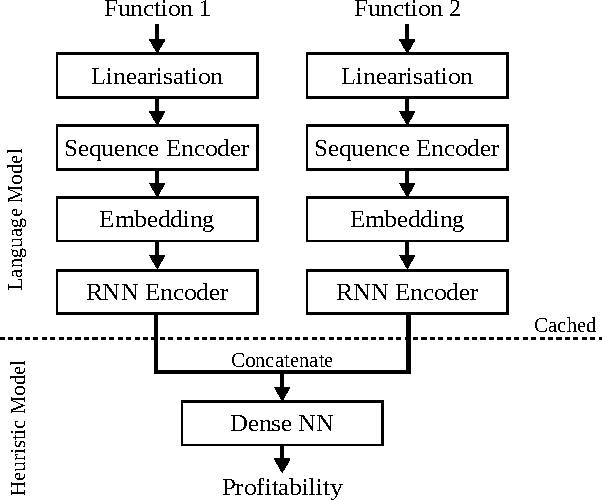
\includegraphics[]{figs/deeplearning-architecture.pdf}
  \caption{
      The proposed deep-learning model architecture that predicts which pairs of functions will be profitably merged. Code properties are extracted from each function into \textit{context vectors} by the language model.
      These context vectors are cached to be later fed to the heuristic model to produce the final profitability prediction.}
  \label{fig:heuristic-model-architecture}
\end{figure}

Figure~\ref{fig:heuristic-model-architecture} provides an overview of the prediction mechanism.
Our mechanism follows a similar approach to previous deep-learning techniques for tuning compilers~\cite{cummins17, mendis19}.

The same linearised functions used for the merge operations, as described in Chapter~\ref{chp:fm-operation}, are used as input to the prediction model.
First, we use a language model based on recurrent neural networks to encode the input functions into context vectors of fixed size.
These vector encodings can be computed only once per function an cached.
Finally, the context vectors of two input functions are concatenated and fed to a dense deep neural network to classify whether or not those functions are profitably merged.
